\documentclass{exam}
\usepackage{graphicx} % Required for inserting images
\usepackage{amsmath}
\usepackage[left=3cm, right=3cm]{geometry}
\usepackage{multicol}
\usepackage{xcolor}
\usepackage{hyperref}
\usepackage{amssymb}

\printanswers % If you want to print answers
%\noprintanswers % If you don't want to print answers
% Specifies the way question are displayed:
\qformat{\textbf{Question\thequestion}\quad(\thepoints)\hfill}
\usepackage{color} % defines a new color
\definecolor{SolutionColor}{rgb}{0.8,0.9,1} % light blue
\framedsolutions % defines the style of the solution environment
% \framedsolutions % defines the style of the solution environment
% Defines the title of the solution environment:
\renewcommand{\solutiontitle}{\noindent\textbf{Solution:}\par\noindent}


%%%%%% Everything below is to import the .ipynb file into latex:

 \usepackage[breakable]{tcolorbox}
    \usepackage{parskip} % Stop auto-indenting (to mimic markdown behaviour)
    

    % Basic figure setup, for now with no caption control since it's done
    % automatically by Pandoc (which extracts ![](path) syntax from Markdown).
    \usepackage{graphicx}
    % Keep aspect ratio if custom image width or height is specified
    \setkeys{Gin}{keepaspectratio}
    % Maintain compatibility with old templates. Remove in nbconvert 6.0
    \let\Oldincludegraphics\includegraphics
    % Ensure that by default, figures have no caption (until we provide a
    % proper Figure object with a Caption API and a way to capture that
    % in the conversion process - todo).
    \usepackage{caption}
    \DeclareCaptionFormat{nocaption}{}
    \captionsetup{format=nocaption,aboveskip=0pt,belowskip=0pt}

    \usepackage{float}
    \floatplacement{figure}{H} % forces figures to be placed at the correct location
    \usepackage{xcolor} % Allow colors to be defined
    \usepackage{enumerate} % Needed for markdown enumerations to work
    \usepackage{geometry} % Used to adjust the document margins
    \usepackage{amsmath} % Equations
    \usepackage{amssymb} % Equations
    \usepackage{textcomp} % defines textquotesingle
    % Hack from http://tex.stackexchange.com/a/47451/13684:
    \AtBeginDocument{%
        \def\PYZsq{\textquotesingle}% Upright quotes in Pygmentized code
    }
    \usepackage{upquote} % Upright quotes for verbatim code
    \usepackage{eurosym} % defines \euro

    \usepackage{iftex}
    \ifPDFTeX
        \usepackage[T1]{fontenc}
        \IfFileExists{alphabeta.sty}{
              \usepackage{alphabeta}
          }{
              \usepackage[mathletters]{ucs}
              \usepackage[utf8x]{inputenc}
          }
    \else
        \usepackage{fontspec}
        \usepackage{unicode-math}
    \fi

    \usepackage{fancyvrb} % verbatim replacement that allows latex
    \usepackage{grffile} % extends the file name processing of package graphics
                         % to support a larger range
    \makeatletter % fix for old versions of grffile with XeLaTeX
    \@ifpackagelater{grffile}{2019/11/01}
    {
      % Do nothing on new versions
    }
    {
      \def\Gread@@xetex#1{%
        \IfFileExists{"\Gin@base".bb}%
        {\Gread@eps{\Gin@base.bb}}%
        {\Gread@@xetex@aux#1}%
      }
    }
    \makeatother
    \usepackage[Export]{adjustbox} % Used to constrain images to a maximum size
    \adjustboxset{max size={0.9\linewidth}{0.9\paperheight}}

    % The hyperref package gives us a pdf with properly built
    % internal navigation ('pdf bookmarks' for the table of contents,
    % internal cross-reference links, web links for URLs, etc.)
    \usepackage{hyperref}
    % The default LaTeX title has an obnoxious amount of whitespace. By default,
    % titling removes some of it. It also provides customization options.
    \usepackage{titling}
    \usepackage{longtable} % longtable support required by pandoc >1.10
    \usepackage{booktabs}  % table support for pandoc > 1.12.2
    \usepackage{array}     % table support for pandoc >= 2.11.3
    \usepackage{calc}      % table minipage width calculation for pandoc >= 2.11.1
    \usepackage[inline]{enumitem} % IRkernel/repr support (it uses the enumerate* environment)
    \usepackage[normalem]{ulem} % ulem is needed to support strikethroughs (\sout)
                                % normalem makes italics be italics, not underlines
    \usepackage{soul}      % strikethrough (\st) support for pandoc >= 3.0.0
    \usepackage{mathrsfs}
    

    
    % Colors for the hyperref package
    \definecolor{urlcolor}{rgb}{0,.145,.698}
    \definecolor{linkcolor}{rgb}{.71,0.21,0.01}
    \definecolor{citecolor}{rgb}{.12,.54,.11}

    % ANSI colors
    \definecolor{ansi-black}{HTML}{3E424D}
    \definecolor{ansi-black-intense}{HTML}{282C36}
    \definecolor{ansi-red}{HTML}{E75C58}
    \definecolor{ansi-red-intense}{HTML}{B22B31}
    \definecolor{ansi-green}{HTML}{00A250}
    \definecolor{ansi-green-intense}{HTML}{007427}
    \definecolor{ansi-yellow}{HTML}{DDB62B}
    \definecolor{ansi-yellow-intense}{HTML}{B27D12}
    \definecolor{ansi-blue}{HTML}{208FFB}
    \definecolor{ansi-blue-intense}{HTML}{0065CA}
    \definecolor{ansi-magenta}{HTML}{D160C4}
    \definecolor{ansi-magenta-intense}{HTML}{A03196}
    \definecolor{ansi-cyan}{HTML}{60C6C8}
    \definecolor{ansi-cyan-intense}{HTML}{258F8F}
    \definecolor{ansi-white}{HTML}{C5C1B4}
    \definecolor{ansi-white-intense}{HTML}{A1A6B2}
    \definecolor{ansi-default-inverse-fg}{HTML}{FFFFFF}
    \definecolor{ansi-default-inverse-bg}{HTML}{000000}

    % common color for the border for error outputs.
    \definecolor{outerrorbackground}{HTML}{FFDFDF}

    % commands and environments needed by pandoc snippets
    % extracted from the output of `pandoc -s`
    \providecommand{\tightlist}{%
      \setlength{\itemsep}{0pt}\setlength{\parskip}{0pt}}
    \DefineVerbatimEnvironment{Highlighting}{Verbatim}{commandchars=\\\{\}}
    % Add ',fontsize=\small' for more characters per line
    \newenvironment{Shaded}{}{}
    \newcommand{\KeywordTok}[1]{\textcolor[rgb]{0.00,0.44,0.13}{\textbf{{#1}}}}
    \newcommand{\DataTypeTok}[1]{\textcolor[rgb]{0.56,0.13,0.00}{{#1}}}
    \newcommand{\DecValTok}[1]{\textcolor[rgb]{0.25,0.63,0.44}{{#1}}}
    \newcommand{\BaseNTok}[1]{\textcolor[rgb]{0.25,0.63,0.44}{{#1}}}
    \newcommand{\FloatTok}[1]{\textcolor[rgb]{0.25,0.63,0.44}{{#1}}}
    \newcommand{\CharTok}[1]{\textcolor[rgb]{0.25,0.44,0.63}{{#1}}}
    \newcommand{\StringTok}[1]{\textcolor[rgb]{0.25,0.44,0.63}{{#1}}}
    \newcommand{\CommentTok}[1]{\textcolor[rgb]{0.38,0.63,0.69}{\textit{{#1}}}}
    \newcommand{\OtherTok}[1]{\textcolor[rgb]{0.00,0.44,0.13}{{#1}}}
    \newcommand{\AlertTok}[1]{\textcolor[rgb]{1.00,0.00,0.00}{\textbf{{#1}}}}
    \newcommand{\FunctionTok}[1]{\textcolor[rgb]{0.02,0.16,0.49}{{#1}}}
    \newcommand{\RegionMarkerTok}[1]{{#1}}
    \newcommand{\ErrorTok}[1]{\textcolor[rgb]{1.00,0.00,0.00}{\textbf{{#1}}}}
    \newcommand{\NormalTok}[1]{{#1}}

    % Additional commands for more recent versions of Pandoc
    \newcommand{\ConstantTok}[1]{\textcolor[rgb]{0.53,0.00,0.00}{{#1}}}
    \newcommand{\SpecialCharTok}[1]{\textcolor[rgb]{0.25,0.44,0.63}{{#1}}}
    \newcommand{\VerbatimStringTok}[1]{\textcolor[rgb]{0.25,0.44,0.63}{{#1}}}
    \newcommand{\SpecialStringTok}[1]{\textcolor[rgb]{0.73,0.40,0.53}{{#1}}}
    \newcommand{\ImportTok}[1]{{#1}}
    \newcommand{\DocumentationTok}[1]{\textcolor[rgb]{0.73,0.13,0.13}{\textit{{#1}}}}
    \newcommand{\AnnotationTok}[1]{\textcolor[rgb]{0.38,0.63,0.69}{\textbf{\textit{{#1}}}}}
    \newcommand{\CommentVarTok}[1]{\textcolor[rgb]{0.38,0.63,0.69}{\textbf{\textit{{#1}}}}}
    \newcommand{\VariableTok}[1]{\textcolor[rgb]{0.10,0.09,0.49}{{#1}}}
    \newcommand{\ControlFlowTok}[1]{\textcolor[rgb]{0.00,0.44,0.13}{\textbf{{#1}}}}
    \newcommand{\OperatorTok}[1]{\textcolor[rgb]{0.40,0.40,0.40}{{#1}}}
    \newcommand{\BuiltInTok}[1]{{#1}}
    \newcommand{\ExtensionTok}[1]{{#1}}
    \newcommand{\PreprocessorTok}[1]{\textcolor[rgb]{0.74,0.48,0.00}{{#1}}}
    \newcommand{\AttributeTok}[1]{\textcolor[rgb]{0.49,0.56,0.16}{{#1}}}
    \newcommand{\InformationTok}[1]{\textcolor[rgb]{0.38,0.63,0.69}{\textbf{\textit{{#1}}}}}
    \newcommand{\WarningTok}[1]{\textcolor[rgb]{0.38,0.63,0.69}{\textbf{\textit{{#1}}}}}


    % Define a nice break command that doesn't care if a line doesn't already
    % exist.
    \def\br{\hspace*{\fill} \\* }
    % Math Jax compatibility definitions
    \def\gt{>}
    \def\lt{<}
    \let\Oldtex\TeX
    \let\Oldlatex\LaTeX
    \renewcommand{\TeX}{\textrm{\Oldtex}}
    \renewcommand{\LaTeX}{\textrm{\Oldlatex}}
    % Document parameters
    % Document title
    \title{Data\_Analysis\_Solutions}
    
    
    
    
    
    
    
% Pygments definitions
\makeatletter
\def\PY@reset{\let\PY@it=\relax \let\PY@bf=\relax%
    \let\PY@ul=\relax \let\PY@tc=\relax%
    \let\PY@bc=\relax \let\PY@ff=\relax}
\def\PY@tok#1{\csname PY@tok@#1\endcsname}
\def\PY@toks#1+{\ifx\relax#1\empty\else%
    \PY@tok{#1}\expandafter\PY@toks\fi}
\def\PY@do#1{\PY@bc{\PY@tc{\PY@ul{%
    \PY@it{\PY@bf{\PY@ff{#1}}}}}}}
\def\PY#1#2{\PY@reset\PY@toks#1+\relax+\PY@do{#2}}

\@namedef{PY@tok@w}{\def\PY@tc##1{\textcolor[rgb]{0.73,0.73,0.73}{##1}}}
\@namedef{PY@tok@c}{\let\PY@it=\textit\def\PY@tc##1{\textcolor[rgb]{0.24,0.48,0.48}{##1}}}
\@namedef{PY@tok@cp}{\def\PY@tc##1{\textcolor[rgb]{0.61,0.40,0.00}{##1}}}
\@namedef{PY@tok@k}{\let\PY@bf=\textbf\def\PY@tc##1{\textcolor[rgb]{0.00,0.50,0.00}{##1}}}
\@namedef{PY@tok@kp}{\def\PY@tc##1{\textcolor[rgb]{0.00,0.50,0.00}{##1}}}
\@namedef{PY@tok@kt}{\def\PY@tc##1{\textcolor[rgb]{0.69,0.00,0.25}{##1}}}
\@namedef{PY@tok@o}{\def\PY@tc##1{\textcolor[rgb]{0.40,0.40,0.40}{##1}}}
\@namedef{PY@tok@ow}{\let\PY@bf=\textbf\def\PY@tc##1{\textcolor[rgb]{0.67,0.13,1.00}{##1}}}
\@namedef{PY@tok@nb}{\def\PY@tc##1{\textcolor[rgb]{0.00,0.50,0.00}{##1}}}
\@namedef{PY@tok@nf}{\def\PY@tc##1{\textcolor[rgb]{0.00,0.00,1.00}{##1}}}
\@namedef{PY@tok@nc}{\let\PY@bf=\textbf\def\PY@tc##1{\textcolor[rgb]{0.00,0.00,1.00}{##1}}}
\@namedef{PY@tok@nn}{\let\PY@bf=\textbf\def\PY@tc##1{\textcolor[rgb]{0.00,0.00,1.00}{##1}}}
\@namedef{PY@tok@ne}{\let\PY@bf=\textbf\def\PY@tc##1{\textcolor[rgb]{0.80,0.25,0.22}{##1}}}
\@namedef{PY@tok@nv}{\def\PY@tc##1{\textcolor[rgb]{0.10,0.09,0.49}{##1}}}
\@namedef{PY@tok@no}{\def\PY@tc##1{\textcolor[rgb]{0.53,0.00,0.00}{##1}}}
\@namedef{PY@tok@nl}{\def\PY@tc##1{\textcolor[rgb]{0.46,0.46,0.00}{##1}}}
\@namedef{PY@tok@ni}{\let\PY@bf=\textbf\def\PY@tc##1{\textcolor[rgb]{0.44,0.44,0.44}{##1}}}
\@namedef{PY@tok@na}{\def\PY@tc##1{\textcolor[rgb]{0.41,0.47,0.13}{##1}}}
\@namedef{PY@tok@nt}{\let\PY@bf=\textbf\def\PY@tc##1{\textcolor[rgb]{0.00,0.50,0.00}{##1}}}
\@namedef{PY@tok@nd}{\def\PY@tc##1{\textcolor[rgb]{0.67,0.13,1.00}{##1}}}
\@namedef{PY@tok@s}{\def\PY@tc##1{\textcolor[rgb]{0.73,0.13,0.13}{##1}}}
\@namedef{PY@tok@sd}{\let\PY@it=\textit\def\PY@tc##1{\textcolor[rgb]{0.73,0.13,0.13}{##1}}}
\@namedef{PY@tok@si}{\let\PY@bf=\textbf\def\PY@tc##1{\textcolor[rgb]{0.64,0.35,0.47}{##1}}}
\@namedef{PY@tok@se}{\let\PY@bf=\textbf\def\PY@tc##1{\textcolor[rgb]{0.67,0.36,0.12}{##1}}}
\@namedef{PY@tok@sr}{\def\PY@tc##1{\textcolor[rgb]{0.64,0.35,0.47}{##1}}}
\@namedef{PY@tok@ss}{\def\PY@tc##1{\textcolor[rgb]{0.10,0.09,0.49}{##1}}}
\@namedef{PY@tok@sx}{\def\PY@tc##1{\textcolor[rgb]{0.00,0.50,0.00}{##1}}}
\@namedef{PY@tok@m}{\def\PY@tc##1{\textcolor[rgb]{0.40,0.40,0.40}{##1}}}
\@namedef{PY@tok@gh}{\let\PY@bf=\textbf\def\PY@tc##1{\textcolor[rgb]{0.00,0.00,0.50}{##1}}}
\@namedef{PY@tok@gu}{\let\PY@bf=\textbf\def\PY@tc##1{\textcolor[rgb]{0.50,0.00,0.50}{##1}}}
\@namedef{PY@tok@gd}{\def\PY@tc##1{\textcolor[rgb]{0.63,0.00,0.00}{##1}}}
\@namedef{PY@tok@gi}{\def\PY@tc##1{\textcolor[rgb]{0.00,0.52,0.00}{##1}}}
\@namedef{PY@tok@gr}{\def\PY@tc##1{\textcolor[rgb]{0.89,0.00,0.00}{##1}}}
\@namedef{PY@tok@ge}{\let\PY@it=\textit}
\@namedef{PY@tok@gs}{\let\PY@bf=\textbf}
\@namedef{PY@tok@ges}{\let\PY@bf=\textbf\let\PY@it=\textit}
\@namedef{PY@tok@gp}{\let\PY@bf=\textbf\def\PY@tc##1{\textcolor[rgb]{0.00,0.00,0.50}{##1}}}
\@namedef{PY@tok@go}{\def\PY@tc##1{\textcolor[rgb]{0.44,0.44,0.44}{##1}}}
\@namedef{PY@tok@gt}{\def\PY@tc##1{\textcolor[rgb]{0.00,0.27,0.87}{##1}}}
\@namedef{PY@tok@err}{\def\PY@bc##1{{\setlength{\fboxsep}{\string -\fboxrule}\fcolorbox[rgb]{1.00,0.00,0.00}{1,1,1}{\strut ##1}}}}
\@namedef{PY@tok@kc}{\let\PY@bf=\textbf\def\PY@tc##1{\textcolor[rgb]{0.00,0.50,0.00}{##1}}}
\@namedef{PY@tok@kd}{\let\PY@bf=\textbf\def\PY@tc##1{\textcolor[rgb]{0.00,0.50,0.00}{##1}}}
\@namedef{PY@tok@kn}{\let\PY@bf=\textbf\def\PY@tc##1{\textcolor[rgb]{0.00,0.50,0.00}{##1}}}
\@namedef{PY@tok@kr}{\let\PY@bf=\textbf\def\PY@tc##1{\textcolor[rgb]{0.00,0.50,0.00}{##1}}}
\@namedef{PY@tok@bp}{\def\PY@tc##1{\textcolor[rgb]{0.00,0.50,0.00}{##1}}}
\@namedef{PY@tok@fm}{\def\PY@tc##1{\textcolor[rgb]{0.00,0.00,1.00}{##1}}}
\@namedef{PY@tok@vc}{\def\PY@tc##1{\textcolor[rgb]{0.10,0.09,0.49}{##1}}}
\@namedef{PY@tok@vg}{\def\PY@tc##1{\textcolor[rgb]{0.10,0.09,0.49}{##1}}}
\@namedef{PY@tok@vi}{\def\PY@tc##1{\textcolor[rgb]{0.10,0.09,0.49}{##1}}}
\@namedef{PY@tok@vm}{\def\PY@tc##1{\textcolor[rgb]{0.10,0.09,0.49}{##1}}}
\@namedef{PY@tok@sa}{\def\PY@tc##1{\textcolor[rgb]{0.73,0.13,0.13}{##1}}}
\@namedef{PY@tok@sb}{\def\PY@tc##1{\textcolor[rgb]{0.73,0.13,0.13}{##1}}}
\@namedef{PY@tok@sc}{\def\PY@tc##1{\textcolor[rgb]{0.73,0.13,0.13}{##1}}}
\@namedef{PY@tok@dl}{\def\PY@tc##1{\textcolor[rgb]{0.73,0.13,0.13}{##1}}}
\@namedef{PY@tok@s2}{\def\PY@tc##1{\textcolor[rgb]{0.73,0.13,0.13}{##1}}}
\@namedef{PY@tok@sh}{\def\PY@tc##1{\textcolor[rgb]{0.73,0.13,0.13}{##1}}}
\@namedef{PY@tok@s1}{\def\PY@tc##1{\textcolor[rgb]{0.73,0.13,0.13}{##1}}}
\@namedef{PY@tok@mb}{\def\PY@tc##1{\textcolor[rgb]{0.40,0.40,0.40}{##1}}}
\@namedef{PY@tok@mf}{\def\PY@tc##1{\textcolor[rgb]{0.40,0.40,0.40}{##1}}}
\@namedef{PY@tok@mh}{\def\PY@tc##1{\textcolor[rgb]{0.40,0.40,0.40}{##1}}}
\@namedef{PY@tok@mi}{\def\PY@tc##1{\textcolor[rgb]{0.40,0.40,0.40}{##1}}}
\@namedef{PY@tok@il}{\def\PY@tc##1{\textcolor[rgb]{0.40,0.40,0.40}{##1}}}
\@namedef{PY@tok@mo}{\def\PY@tc##1{\textcolor[rgb]{0.40,0.40,0.40}{##1}}}
\@namedef{PY@tok@ch}{\let\PY@it=\textit\def\PY@tc##1{\textcolor[rgb]{0.24,0.48,0.48}{##1}}}
\@namedef{PY@tok@cm}{\let\PY@it=\textit\def\PY@tc##1{\textcolor[rgb]{0.24,0.48,0.48}{##1}}}
\@namedef{PY@tok@cpf}{\let\PY@it=\textit\def\PY@tc##1{\textcolor[rgb]{0.24,0.48,0.48}{##1}}}
\@namedef{PY@tok@c1}{\let\PY@it=\textit\def\PY@tc##1{\textcolor[rgb]{0.24,0.48,0.48}{##1}}}
\@namedef{PY@tok@cs}{\let\PY@it=\textit\def\PY@tc##1{\textcolor[rgb]{0.24,0.48,0.48}{##1}}}

\def\PYZbs{\char`\\}
\def\PYZus{\char`\_}
\def\PYZob{\char`\{}
\def\PYZcb{\char`\}}
\def\PYZca{\char`\^}
\def\PYZam{\char`\&}
\def\PYZlt{\char`\<}
\def\PYZgt{\char`\>}
\def\PYZsh{\char`\#}
\def\PYZpc{\char`\%}
\def\PYZdl{\char`\$}
\def\PYZhy{\char`\-}
\def\PYZsq{\char`\'}
\def\PYZdq{\char`\"}
\def\PYZti{\char`\~}
% for compatibility with earlier versions
\def\PYZat{@}
\def\PYZlb{[}
\def\PYZrb{]}
\makeatother


    % For linebreaks inside Verbatim environment from package fancyvrb.
    \makeatletter
        \newbox\Wrappedcontinuationbox
        \newbox\Wrappedvisiblespacebox
        \newcommand*\Wrappedvisiblespace {\textcolor{red}{\textvisiblespace}}
        \newcommand*\Wrappedcontinuationsymbol {\textcolor{red}{\llap{\tiny$\m@th\hookrightarrow$}}}
        \newcommand*\Wrappedcontinuationindent {3ex }
        \newcommand*\Wrappedafterbreak {\kern\Wrappedcontinuationindent\copy\Wrappedcontinuationbox}
        % Take advantage of the already applied Pygments mark-up to insert
        % potential linebreaks for TeX processing.
        %        {, <, #, %, $, ' and ": go to next line.
        %        _, }, ^, &, >, - and ~: stay at end of broken line.
        % Use of \textquotesingle for straight quote.
        \newcommand*\Wrappedbreaksatspecials {%
            \def\PYGZus{\discretionary{\char`\_}{\Wrappedafterbreak}{\char`\_}}%
            \def\PYGZob{\discretionary{}{\Wrappedafterbreak\char`\{}{\char`\{}}%
            \def\PYGZcb{\discretionary{\char`\}}{\Wrappedafterbreak}{\char`\}}}%
            \def\PYGZca{\discretionary{\char`\^}{\Wrappedafterbreak}{\char`\^}}%
            \def\PYGZam{\discretionary{\char`\&}{\Wrappedafterbreak}{\char`\&}}%
            \def\PYGZlt{\discretionary{}{\Wrappedafterbreak\char`\<}{\char`\<}}%
            \def\PYGZgt{\discretionary{\char`\>}{\Wrappedafterbreak}{\char`\>}}%
            \def\PYGZsh{\discretionary{}{\Wrappedafterbreak\char`\#}{\char`\#}}%
            \def\PYGZpc{\discretionary{}{\Wrappedafterbreak\char`\%}{\char`\%}}%
            \def\PYGZdl{\discretionary{}{\Wrappedafterbreak\char`\$}{\char`\$}}%
            \def\PYGZhy{\discretionary{\char`\-}{\Wrappedafterbreak}{\char`\-}}%
            \def\PYGZsq{\discretionary{}{\Wrappedafterbreak\textquotesingle}{\textquotesingle}}%
            \def\PYGZdq{\discretionary{}{\Wrappedafterbreak\char`\"}{\char`\"}}%
            \def\PYGZti{\discretionary{\char`\~}{\Wrappedafterbreak}{\char`\~}}%
        }
        % Some characters . , ; ? ! / are not pygmentized.
        % This macro makes them "active" and they will insert potential linebreaks
        \newcommand*\Wrappedbreaksatpunct {%
            \lccode`\~`\.\lowercase{\def~}{\discretionary{\hbox{\char`\.}}{\Wrappedafterbreak}{\hbox{\char`\.}}}%
            \lccode`\~`\,\lowercase{\def~}{\discretionary{\hbox{\char`\,}}{\Wrappedafterbreak}{\hbox{\char`\,}}}%
            \lccode`\~`\;\lowercase{\def~}{\discretionary{\hbox{\char`\;}}{\Wrappedafterbreak}{\hbox{\char`\;}}}%
            \lccode`\~`\:\lowercase{\def~}{\discretionary{\hbox{\char`\:}}{\Wrappedafterbreak}{\hbox{\char`\:}}}%
            \lccode`\~`\?\lowercase{\def~}{\discretionary{\hbox{\char`\?}}{\Wrappedafterbreak}{\hbox{\char`\?}}}%
            \lccode`\~`\!\lowercase{\def~}{\discretionary{\hbox{\char`\!}}{\Wrappedafterbreak}{\hbox{\char`\!}}}%
            \lccode`\~`\/\lowercase{\def~}{\discretionary{\hbox{\char`\/}}{\Wrappedafterbreak}{\hbox{\char`\/}}}%
            \catcode`\.\active
            \catcode`\,\active
            \catcode`\;\active
            \catcode`\:\active
            \catcode`\?\active
            \catcode`\!\active
            \catcode`\/\active
            \lccode`\~`\~
        }
    \makeatother

    \let\OriginalVerbatim=\Verbatim
    \makeatletter
    \renewcommand{\Verbatim}[1][1]{%
        %\parskip\z@skip
        \sbox\Wrappedcontinuationbox {\Wrappedcontinuationsymbol}%
        \sbox\Wrappedvisiblespacebox {\FV@SetupFont\Wrappedvisiblespace}%
        \def\FancyVerbFormatLine ##1{\hsize\linewidth
            \vtop{\raggedright\hyphenpenalty\z@\exhyphenpenalty\z@
                \doublehyphendemerits\z@\finalhyphendemerits\z@
                \strut ##1\strut}%
        }%
        % If the linebreak is at a space, the latter will be displayed as visible
        % space at end of first line, and a continuation symbol starts next line.
        % Stretch/shrink are however usually zero for typewriter font.
        \def\FV@Space {%
            \nobreak\hskip\z@ plus\fontdimen3\font minus\fontdimen4\font
            \discretionary{\copy\Wrappedvisiblespacebox}{\Wrappedafterbreak}
            {\kern\fontdimen2\font}%
        }%

        % Allow breaks at special characters using \PYG... macros.
        \Wrappedbreaksatspecials
        % Breaks at punctuation characters . , ; ? ! and / need catcode=\active
        \OriginalVerbatim[#1,codes*=\Wrappedbreaksatpunct]%
    }
    \makeatother

    % Exact colors from NB
    \definecolor{incolor}{HTML}{303F9F}
    \definecolor{outcolor}{HTML}{D84315}
    \definecolor{cellborder}{HTML}{CFCFCF}
    \definecolor{cellbackground}{HTML}{F7F7F7}

    % prompt
    \makeatletter
    \newcommand{\boxspacing}{\kern\kvtcb@left@rule\kern\kvtcb@boxsep}
    \makeatother
    \newcommand{\prompt}[4]{
        {\ttfamily\llap{{\color{#2}[#3]:\hspace{3pt}#4}}\vspace{-\baselineskip}}
    }
    

    
    % Prevent overflowing lines due to hard-to-break entities
    \sloppy
    % Setup hyperref package
    \hypersetup{
      breaklinks=true,  % so long urls are correctly broken across lines
      colorlinks=true,
      urlcolor=urlcolor,
      linkcolor=linkcolor,
      citecolor=citecolor,
      }
    % Slightly bigger margins than the latex defaults
    
    \geometry{verbose,tmargin=1in,bmargin=1in,lmargin=1in,rmargin=1in}





\title{Miscellaneous problems}
\date{}
\author{Raphael Kelly, Sven Bachmann, and Peter Harrington}

\begin{document}

\maketitle

\section{Carbon flux}
\subsection*{Question 1}
\label{q1}

The Mauna Loa observatory has been measuring the atmospheric makeup of Earth since 1958. As part of ongoing research projects, the Mauna Loa observatory collects monthly averaged data on the concentration of $CO_2$ in the atmosphere near its observation point. The data is shown below for the year 2022.

\begin{center}
        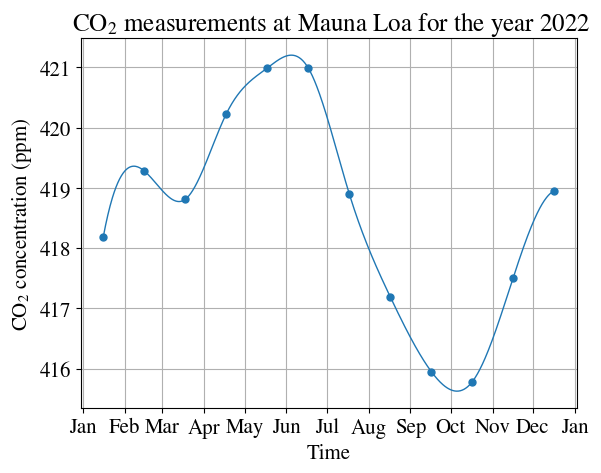
\includegraphics[scale=0.7]{co2measurementsmaunoloa.png}
        
        \textbf{Figure 1.} Graph showing the concentration of $CO_2$ for different months in 2022. Markers represent data. A curve was fitted between datapoints to show continuity. Data source is \url{https://gml.noaa.gov/ccgg/trends/data.html}.
        \end{center}

\begin{enumerate}
    \item
        Let $C(t)$ be the concentration of $CO_2$. The net flux is defined as the time-derivative of the $CO_2$ concentration, $\frac{dC}{dt}$. \textbf{Which} of the graphs in Figure 2. accurately represents the net flux in the $CO_2$ concentration with respect to time?

    \begin{center}
        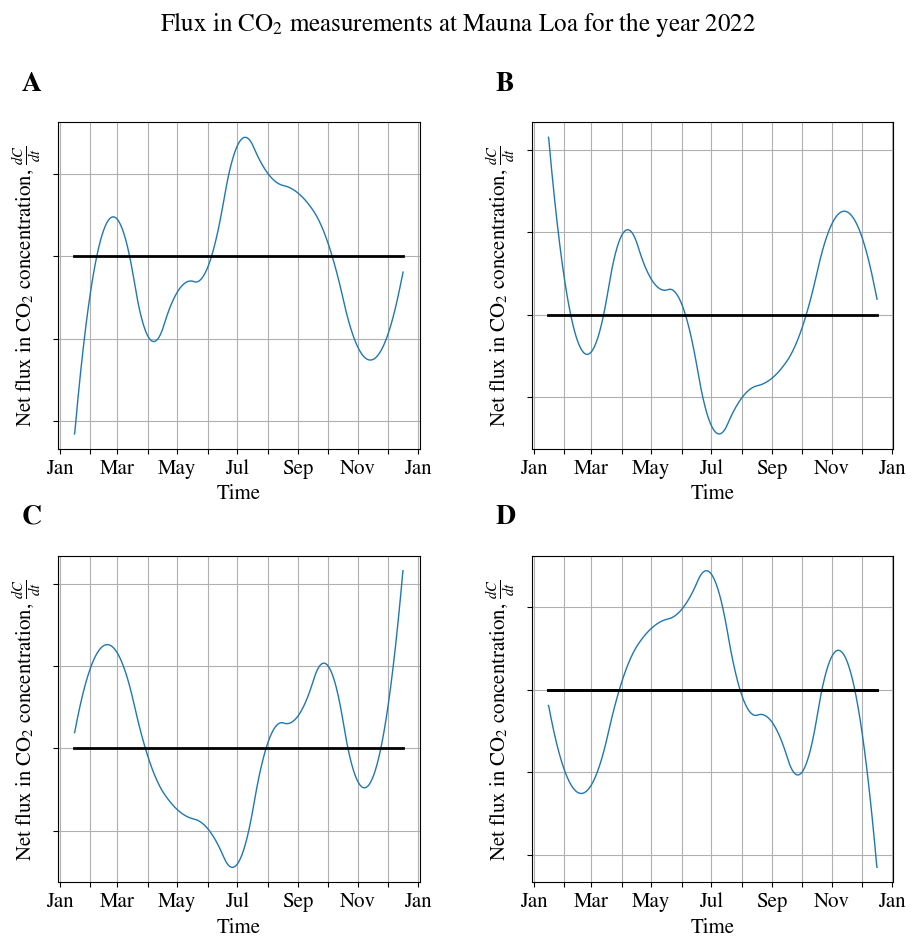
\includegraphics[scale=0.6]{fluxco2measurementamaunaloa.png}
        
        \textbf{Figure 2.} Potential graphs of the net flux in $CO_2$ concentration in 2022.
    \end{center}



    \item In practice, the net flux is a combination of various effects, some contributing to an increase in the $CO_2$ concentration called the influx, others contributing to a decrease in the $CO_2$ concentration called the outflux. \textbf{During which} months is there a point in time at which carbon influx matches outflux? 


\end{enumerate}




\subsection*{Question 2}
\label{q2}

%The solubility, $S$, of $CO_2$ in water goes down if the temperature $T$ of water goes up. The concentration of $CO_2$ in water $C$ goes up if the solubility, $S$, increases.
At equilibrium, a fraction of $CO_2$ is dissolved in water. In order to discuss this effect, we consider three variables: $T$ for the temperature, $C$ for the concentration of $CO_2$, and $S$ for the solubility. The solubility characterizes the ability of a substance (here $CO_2$) to form a solution with another substance (here water). All other parameters being constant, increasing the solubility will increase the concentration. Physical processes are so that, all other parameters being constant, solubility decreases as temperature increases.

\begin{enumerate}
    \item Is $\frac{dS}{dT}$ positive or negative?
    \item Is $\frac{dC}{dS}$ positive or negative?
    \item Is $\frac{dC}{dT}$ positive or negative?
\end{enumerate}





%Based on http://maecourses.ucsd.edu/MAE119/WI_2018/ewExternalFiles/Carbon%20Budget%20Homework%20from%20Ft%20Bend.pdf.

\section{Solar radiation}

\subsection*{Question 1}

\begin{enumerate}
    \item Consider the Earth to be a perfect sphere of radius $r$. The Sun has a diameter of 109 times the Earth, so light rays incident upon the Earth from the Sun are approximately parallel to each other. Assume the Earth has no axial tilt. Consider the diagram shown below.

    \begin{centering}
        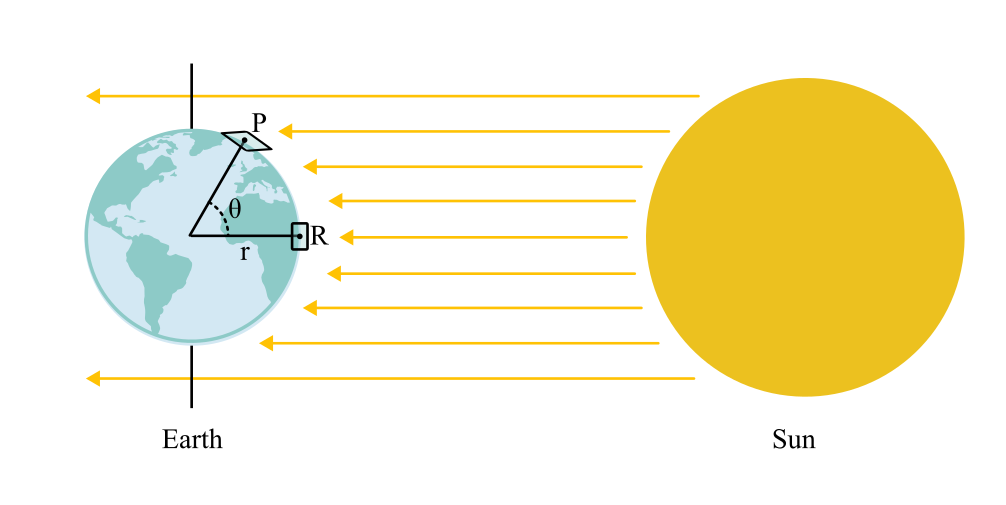
\includegraphics[scale=1]{sunrayqa.png}
    \end{centering}
 
    Consider a stationary Earth with a vertical, non-tilted axis of rotation. At a point $R$ on the equator, the solar rays are perpendicular to the Earth’s surface, so the energy received is equal to the solar constant, $Q=1.361 kWm^{-2}$. Consider a point $P$ at the same longitude as $R$, but at an angle $\theta$ away from $R$, for $\theta \in [-\pi,\pi]$. Let $E( \theta )$ be the amount of solar energy that reaches $1m^2$ of on Earth at an angle $\theta$ away from the point $R$. %At 12pm, proportionally less solar energy is arriving per $m^{2}$ at point $P$ because the surface of the Earth is tilted.
    
    \begin{enumerate}
        \item \textbf{Determine} $E(\theta)$ ensuring that your function is accurate across the entire domain $\theta \in [-\pi,\pi]$.

 
    
        \item The total amount of solar energy arriving at the Earth is $Q \pi r^2 \times$ (1.36 $W m^{-2}$), where $r$ is the radius of the Earth. Use this information to \textbf{determine} the average amount of solar radiation reaching each meter squared on the surface of the Earth.



        \item For some angle $\theta_c$, the amount of solar energy received per $m^2$ at point $P$ when $\theta=\theta_c$ is exactly equal to the average amount of solar energy per squared meter across the entire Earth. Determine $\theta_c$.

    
    \end{enumerate}

\subsection*{Extensions to question 1}
    
    
    \begin{enumerate}
        \item We will consider the rotation of the Earth by considering a second dimension, and utilizing the time $t$ in days. Consider the graphic below.
        
        \begin{centering}
        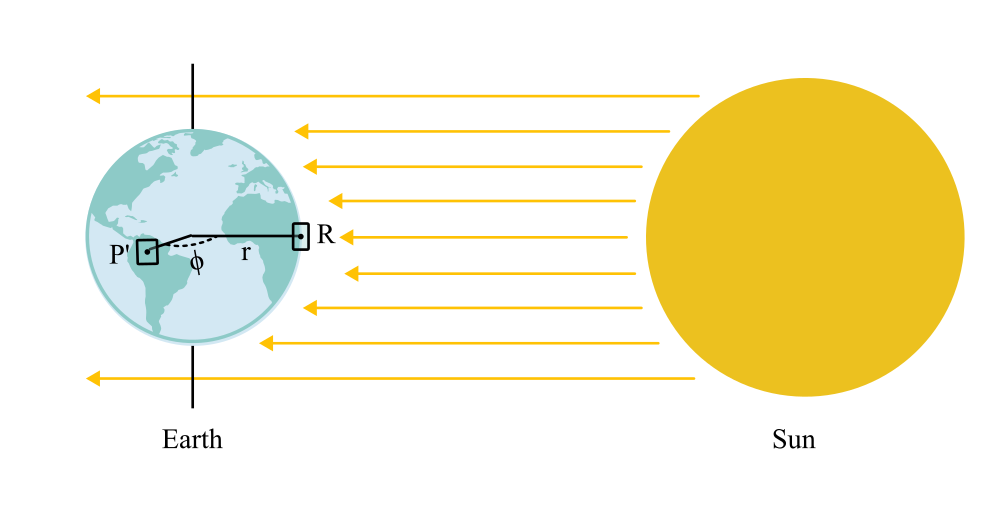
\includegraphics[scale=1]{sunrayqd.png}
        \end{centering}
        
        In this case, the amount of Energy reaching the Earth at point $P'$ is a function of the angle $\phi \in [0, 2\pi]$ relative to point $R$. Since the Earth makes a full rotation in $1$ day, we will use the function $\phi = 2\pi t$ to represent the relationship between these two variables. Now, the term $F(t)$ is defined to be the fraction of the energy at the same latitude $E(\theta)$ that is absorbed by each square meter of the Earth as a function of the time of day $t$. \textbf{Construct} an expression for $F(t)$, ensuring that it is valid for the entire domain $t \in [0,1]$.



        \item The function $E_T= E(\theta)F(t)/Q$ represents the total amount of energy experienced at any latitude of the Earth at any particular time. $E_T(\theta, t)$ is a function of two variables. There is only one critical point of this function for which $E_T \neq 0$. Find this non-zero critical point and classify it as a max, min, or saddle.
        


    
        \item 
    
        \begin{centering}
            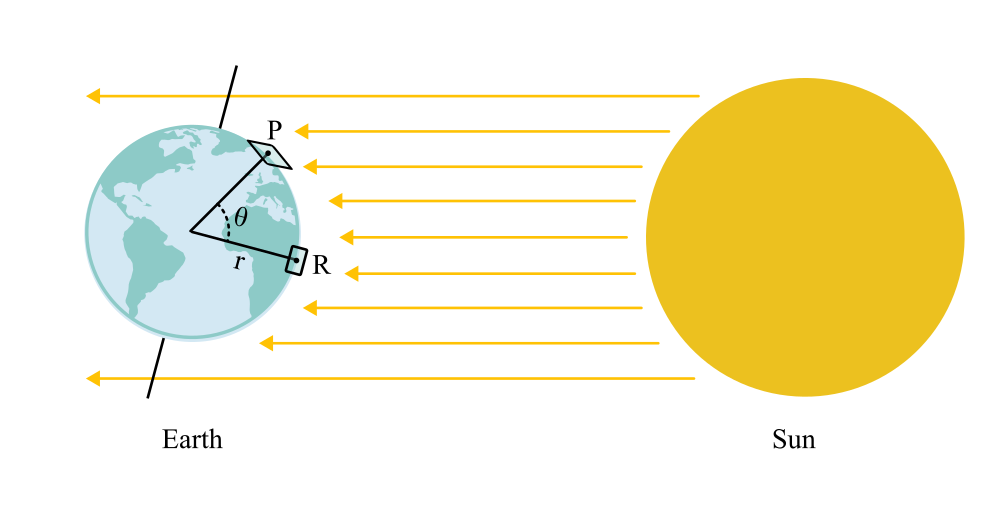
\includegraphics[scale=1]{sunrayqb.png}
        \end{centering}
        
        Consider an altered graphic, which represents the same situation as in a) (before the extension questions), except with the Earth having an axial tilt of $23.4^\circ$ relative to the vertical. The point where light incident upon the Earth is at a maximum now sits at an angle of $\theta=23.4^\circ$. 
        
        \textbf{Determine} a new expression for $E(\theta)$, representing the amount of solar energy reaching each square meter of the Earth where $\theta$ is now given in degress, still ensuring that your function is accurate across the entire domain $\theta \in (-180,180)$ degrees.
        


        
    \end{enumerate}

    %Earth tilt. Curvature. Seasons... Add it to E... a different function of t...
    
\end{enumerate}

\newpage

\section{Glaciers}


Glaciers play a critical role in maintaining the energy balance of the Earth. A climate scientist is studying the effect that solar energy has on the geometry of glacier. Because glaciers are made of water, they are susceptible to melting from solar energy, which can cause viscous flow to alter its shape over time. This scientist has decided to create a 3D model of the edge of a glacier. A graphical representation of the shape of this object is displayed in \textbf{Figure \ref{fig:glacier}}.

\begin{figure}[ht]
    \centering
    \includegraphics[width=\linewidth]{Miscellaneous/glaciericevolume.png}
    \caption{ Diagram showing the shape of a 3D model of the edge of a glacier: a) shows the final 3D shape, b) shows the side-portrait view of the 3D shape at $z=0$, and c) shows a top-down view of the edge of the 3D shape.}
    \label{fig:glacier}
\end{figure}



%\vspace{5mm}

%\fcolorbox{white}{white}{ %first box black for border
%\minipage[t]{\dimexpr0.93\linewidth-3\fboxsep-4\fboxrule\relax}

%\begin{center}%
%    \includegraphics[scale=0.8]{glaciericevolume.png}
    
%    \raggedright \textbf{Figure 1.} Diagram showing the shape of a 3D model of the edge of a glacier. 
%    \begin{enumerate}[label=\alph*)]
%        \item shows the final 3D shape.
%        \item shows the side-portrait view of the 3D %shape at $z=0$.
 %%       \item shows a top-down view of the edge of the 3D shape.
 %   \end{enumerate}
%\end{center}%

%\endminipage} 

\vspace{5mm}


\noindent The shape of this model can be reconstructed by cutting the 3D shape into infinitely many 2D slices of the same shape in the $xy$ plane, and then stacking these slices along the $z$ axis. Consider a 3D coordinate plane with an $x$, $y$, and $z$ axis.
\begin{itemize}
    \item The length of the entire shape (in the $z$-direction) is given by $l$.
    \item The width of the entire shape (in the $x$-direction) is given by $w$.
    \item The height of the entire shape (in the $y$-direction) is given by $h$.
\end{itemize}
Further, consider the following information.
\begin{itemize}
    \item Each 2D slice has the same proportions, but a different size. The shape of each slice is given by the area under the curve of $$y=H(z)\cos \left(\frac{\pi x}{2 W(z)} \right) \qquad x \in [0,W(z)],$$ where $H(z)$ and $W(z)$ are the height and width of a specific slice along the $z$ axis.
    \item When $z=0$, the shape of the slice is given by the area under the curve of $$y=h\cos \left(\frac{\pi x}{2 w} \right) \qquad x \in [0,w].$$
    \item Each 2D slice is placed orthogonal to the $z$-axis. The corner of every slice sits on the $z$-axis.
    \item The width of each slice, $W(z)$, depends on the value of $z$. $W(z)$ and $z$ always obey the following relationship: $$\left(\frac{W(z)}{w}\right)^2+\left(\frac{2z}{l}\right)^4=1.$$
\end{itemize}

\subsection*{Part A}

\begin{enumerate}
    \item \textbf{Determine} an expression for the area of each 2D slice in terms of $h$, $w$, and $W(z)$.


    \item \textbf{Determine} an expression for the total volume of this shape in terms of $h$, $w$, and $l$.



    
\end{enumerate}

\subsection*{Part B}

\begin{enumerate}
    \item Let $t$ be the time in years. A simulation is being performed using the 3D model.  Assuming that both the length and volume of the glacier remain constant then if the height of the glacier edge decreases by 10$\rm m/yr$ (i.e. $\frac{dh}{dt}=-0.01$), \textbf{determine} the rate the width will change, $\frac{dw}{dt}$, when $h$ is 2.1 km, $l$ is 20.0 km, and $w$ is 9.0 km. (Note for instructors: if Part B is done separately from Part A, then the volume of the glacier should be given).



    \item Another simulation is performed with the same initial conditions, but only the volume is constant. If $\frac{dl}{dt}=0.025$ and $\frac{dw}{dt}=0.033$, \textbf{determine}  the rate the height is changing, $\frac{dh}{dt}$, when $h$ is 2.1 km, $l$ is 20.0 km, and $w$ is 9.0 km.



    \item Another simulation is performed with the same initial conditions, but only the volume is held constant. If $\frac{dh}{dt}=-0.005$ and $\frac{dw}{dt}=\frac{dl}{dt}$, \textbf{determine} the rate the width of the glacier is changing, $\frac{dw}{dt}$, when $h$ is 2.1 km, $l$ is 20.0 km, and $w$ is 9.0 km.



    \item Another simulation is performed with the same initial conditions, but no variables are constant. Let the volume of the solid be $V$. If $\frac{dh}{dt}=-0.005$, $\frac{dw}{dt}=0.02$,  and $\frac{dl}{dt}=0.034$, \textbf{determine} the rate the volume of the glacier is changing $\frac{dV}{dt}$, when $h$ is 2.1 km, $l$ is 20.0 km, and $w$ is 9.0 km.


    
\end{enumerate}


\section{Numerical extension to Math 100 EBM assignment (run on syzygy)}\label{energy-balance-model-numerical-exploration-designed-to-accompany-math-100-assignment}

(.ipynb file can be found in folder. If you make changes to ipynb file, you can run `jupyter nbconvert --to latex Data\_Analysis\_Questions.ipynb' in the UBC syzygy terminal to export assignment to latex)



    The code below imports and creates the functions you need for this
assignment. Run the code block below before continuing to the
assignment, but do not edit it.

    \begin{tcolorbox}[breakable, size=fbox, boxrule=1pt, pad at break*=1mm,colback=cellbackground, colframe=cellborder]
\prompt{In}{incolor}{29}{\boxspacing}
\begin{Verbatim}[commandchars=\\\{\}]
\PY{c+c1}{\PYZsh{} DO NOT EDIT}

\PY{c+c1}{\PYZsh{} Imports}

\PY{k+kn}{import} \PY{n+nn}{matplotlib}
\PY{k+kn}{import} \PY{n+nn}{math}
\PY{k+kn}{import} \PY{n+nn}{numpy} \PY{k}{as} \PY{n+nn}{np}
\PY{k+kn}{import} \PY{n+nn}{matplotlib}\PY{n+nn}{.}\PY{n+nn}{pyplot} \PY{k}{as} \PY{n+nn}{plt}
\PY{k+kn}{from} \PY{n+nn}{scipy} \PY{k+kn}{import} \PY{n}{integrate}
\PY{n}{matplotlib}\PY{o}{.}\PY{n}{rcParams}\PY{p}{[}\PY{l+s+s1}{\PYZsq{}}\PY{l+s+s1}{mathtext.fontset}\PY{l+s+s1}{\PYZsq{}}\PY{p}{]} \PY{o}{=} \PY{l+s+s1}{\PYZsq{}}\PY{l+s+s1}{stix}\PY{l+s+s1}{\PYZsq{}}
\PY{n}{matplotlib}\PY{o}{.}\PY{n}{rcParams}\PY{p}{[}\PY{l+s+s1}{\PYZsq{}}\PY{l+s+s1}{font.family}\PY{l+s+s1}{\PYZsq{}}\PY{p}{]} \PY{o}{=} \PY{l+s+s1}{\PYZsq{}}\PY{l+s+s1}{STIXGeneral}\PY{l+s+s1}{\PYZsq{}}
\PY{c+c1}{\PYZsh{}matplotlib.pyplot.title(r\PYZsq{}ABC123 vs \PYZdl{}\PYZbs{}mathrm\PYZob{}ABC123\PYZcb{}\PYZca{}\PYZob{}123\PYZcb{}\PYZdl{}\PYZsq{})}
\PY{n}{matplotlib}\PY{o}{.}\PY{n}{rcParams}\PY{o}{.}\PY{n}{update}\PY{p}{(}\PY{p}{\PYZob{}}\PY{l+s+s1}{\PYZsq{}}\PY{l+s+s1}{font.size}\PY{l+s+s1}{\PYZsq{}}\PY{p}{:} \PY{l+m+mi}{15}\PY{p}{\PYZcb{}}\PY{p}{)}

\PY{c+c1}{\PYZsh{} Albedo Functions}

\PY{k}{def} \PY{n+nf}{albedo1}\PY{p}{(}\PY{n}{T}\PY{p}{)}\PY{p}{:}
  \PY{k}{if} \PY{n}{T} \PY{o}{\PYZlt{}}\PY{o}{=} \PY{l+m+mi}{247}\PY{p}{:}
    \PY{k}{return} \PY{l+m+mf}{0.7}
  \PY{k}{elif} \PY{n}{T} \PY{o}{\PYZgt{}}\PY{o}{=} \PY{l+m+mi}{282}\PY{p}{:}
    \PY{k}{return} \PY{l+m+mf}{0.3}
  \PY{k}{else}\PY{p}{:}
    \PY{c+c1}{\PYZsh{}return \PYZhy{}2/175*T+(1233)/350}
    \PY{k}{return} \PY{l+m+mf}{3.52296} \PY{o}{\PYZhy{}} \PY{l+m+mf}{0.011429}\PY{o}{*}\PY{n}{T}

\PY{k}{def} \PY{n+nf}{albedo2}\PY{p}{(}\PY{n}{T}\PY{p}{)}\PY{p}{:}
  \PY{k}{return} \PY{l+m+mf}{0.5}\PY{o}{\PYZhy{}}\PY{l+m+mf}{0.2} \PY{o}{*} \PY{n}{math}\PY{o}{.}\PY{n}{tanh}\PY{p}{(}\PY{p}{(}\PY{n}{T}\PY{o}{\PYZhy{}}\PY{l+m+mi}{265}\PY{p}{)}\PY{o}{/}\PY{l+m+mi}{10}\PY{p}{)}

\PY{k}{def} \PY{n+nf}{albedo3}\PY{p}{(}\PY{n}{T}\PY{p}{)}\PY{p}{:}
  \PY{k}{if} \PY{n}{T} \PY{o}{\PYZlt{}}\PY{o}{=} \PY{l+m+mi}{264}\PY{p}{:}
    \PY{k}{return} \PY{l+m+mf}{0.7}
  \PY{k}{else}\PY{p}{:}
    \PY{k}{return} \PY{l+m+mf}{0.3}

\PY{c+c1}{\PYZsh{} Constants}

\PY{n}{C}\PY{o}{=}\PY{l+m+mf}{1e23}
\PY{n}{r}\PY{o}{=}\PY{l+m+mf}{6.3781e6}
\PY{n}{Q}\PY{o}{=}\PY{l+m+mi}{1365}
\PY{n}{sigma}\PY{o}{=}\PY{l+m+mf}{5.6704e\PYZhy{}8}
\PY{n}{epsilon}\PY{o}{=}\PY{l+m+mf}{0.600}

\PY{c+c1}{\PYZsh{} Initial Conditions}

\PY{n}{T0} \PY{o}{=} \PY{l+m+mf}{232.112}

\PY{c+c1}{\PYZsh{} Differential Equation (Energy Balance Model)}

\PY{k}{def} \PY{n+nf}{dTdt}\PY{p}{(}\PY{n}{t}\PY{p}{,}\PY{n}{T}\PY{p}{)}\PY{p}{:}
  \PY{n}{Ein} \PY{o}{=} \PY{n}{np}\PY{o}{.}\PY{n}{pi}\PY{o}{*}\PY{n}{r}\PY{o}{*}\PY{o}{*}\PY{l+m+mf}{2.0}\PY{o}{*}\PY{n}{Q}\PY{o}{*}\PY{p}{(}\PY{l+m+mi}{1}\PY{o}{\PYZhy{}}\PY{n}{albedo}\PY{p}{(}\PY{n}{T}\PY{p}{)}\PY{p}{)}
  \PY{n}{Eout} \PY{o}{=} \PY{l+m+mf}{4.0}\PY{o}{*}\PY{n}{np}\PY{o}{.}\PY{n}{pi}\PY{o}{*}\PY{n}{r}\PY{o}{*}\PY{o}{*}\PY{l+m+mi}{2}\PY{o}{*}\PY{n}{sigma}\PY{o}{*}\PY{n}{epsilon}\PY{o}{*}\PY{n}{T}\PY{o}{*}\PY{o}{*}\PY{l+m+mi}{4}
  \PY{k}{return} \PY{p}{[}\PY{n}{Ein}\PY{o}{/}\PY{n}{C} \PY{o}{\PYZhy{}} \PY{n}{Eout}\PY{o}{/}\PY{n}{C}\PY{p}{]}

\PY{c+c1}{\PYZsh{} Solving the Equation}

\PY{k}{def} \PY{n+nf}{solveAndGraph}\PY{p}{(}\PY{p}{)}\PY{p}{:}
  \PY{n}{xs} \PY{o}{=} \PY{n}{np}\PY{o}{.}\PY{n}{linspace}\PY{p}{(}\PY{l+m+mi}{220}\PY{p}{,}\PY{l+m+mi}{320}\PY{p}{,}\PY{l+m+mi}{100}\PY{p}{)}
  \PY{n}{ys} \PY{o}{=} \PY{n}{np}\PY{o}{.}\PY{n}{vectorize}\PY{p}{(}\PY{n}{albedo}\PY{p}{)}\PY{p}{(}\PY{n}{xs}\PY{p}{)}
  \PY{n}{plt}\PY{o}{.}\PY{n}{plot}\PY{p}{(}\PY{n}{xs}\PY{p}{,}\PY{n}{ys}\PY{p}{)}
  \PY{n}{plt}\PY{o}{.}\PY{n}{title}\PY{p}{(}\PY{l+s+sa}{r}\PY{l+s+s2}{\PYZdq{}}\PY{l+s+s2}{Albedo \PYZdl{}}\PY{l+s+s2}{\PYZbs{}}\PY{l+s+s2}{alpha(T)\PYZdl{}}\PY{l+s+s2}{\PYZdq{}}\PY{p}{)}
  \PY{n}{plt}\PY{o}{.}\PY{n}{xlabel}\PY{p}{(}\PY{l+s+s2}{\PYZdq{}}\PY{l+s+s2}{Temperature (K)}\PY{l+s+s2}{\PYZdq{}}\PY{p}{)}
  \PY{n}{plt}\PY{o}{.}\PY{n}{ylabel}\PY{p}{(}\PY{l+s+s2}{\PYZdq{}}\PY{l+s+s2}{Albedo (unitless)}\PY{l+s+s2}{\PYZdq{}}\PY{p}{)}
  \PY{n}{plt}\PY{o}{.}\PY{n}{grid}\PY{p}{(}\PY{p}{)}
  \PY{n}{plt}\PY{o}{.}\PY{n}{show}\PY{p}{(}\PY{p}{)}

  \PY{n}{sol} \PY{o}{=} \PY{n}{integrate}\PY{o}{.}\PY{n}{solve\PYZus{}ivp}\PY{p}{(}\PY{n}{dTdt}\PY{p}{,} \PY{p}{[}\PY{l+m+mf}{0.0}\PY{p}{,}\PY{l+m+mf}{3.156e9}\PY{p}{]}\PY{p}{,} \PY{p}{[}\PY{n}{T0}\PY{p}{]}\PY{p}{,} \PY{n}{t\PYZus{}eval}\PY{o}{=}\PY{n}{np}\PY{o}{.}\PY{n}{linspace}\PY{p}{(}\PY{l+m+mi}{0}\PY{p}{,}\PY{l+m+mf}{3.156e9}\PY{p}{,}\PY{l+m+mi}{100}\PY{p}{)}\PY{p}{)}
  \PY{n}{plt}\PY{o}{.}\PY{n}{plot}\PY{p}{(}\PY{n}{sol}\PY{o}{.}\PY{n}{t}\PY{o}{/}\PY{l+m+mf}{3.154e7}\PY{p}{,}\PY{n}{sol}\PY{o}{.}\PY{n}{y}\PY{p}{[}\PY{l+m+mi}{0}\PY{p}{]}\PY{p}{)}
  \PY{n}{plt}\PY{o}{.}\PY{n}{title}\PY{p}{(}\PY{l+s+sa}{r}\PY{l+s+s2}{\PYZdq{}}\PY{l+s+s2}{Temperature vs. Time}\PY{l+s+s2}{\PYZdq{}}\PY{p}{)}
  \PY{n}{plt}\PY{o}{.}\PY{n}{xlabel}\PY{p}{(}\PY{l+s+s2}{\PYZdq{}}\PY{l+s+s2}{Time (years)}\PY{l+s+s2}{\PYZdq{}}\PY{p}{)}
  \PY{n}{plt}\PY{o}{.}\PY{n}{grid}\PY{p}{(}\PY{n}{which}\PY{o}{=}\PY{l+s+s1}{\PYZsq{}}\PY{l+s+s1}{major}\PY{l+s+s1}{\PYZsq{}}\PY{p}{,} \PY{n}{linestyle}\PY{o}{=}\PY{l+s+s1}{\PYZsq{}}\PY{l+s+s1}{\PYZhy{}}\PY{l+s+s1}{\PYZsq{}}\PY{p}{)}
  \PY{n}{plt}\PY{o}{.}\PY{n}{grid}\PY{p}{(}\PY{n}{which}\PY{o}{=}\PY{l+s+s1}{\PYZsq{}}\PY{l+s+s1}{minor}\PY{l+s+s1}{\PYZsq{}}\PY{p}{,} \PY{n}{linestyle}\PY{o}{=}\PY{l+s+s1}{\PYZsq{}}\PY{l+s+s1}{\PYZhy{}}\PY{l+s+s1}{\PYZsq{}}\PY{p}{,} \PY{n}{alpha}\PY{o}{=}\PY{l+m+mf}{0.2}\PY{p}{)}
  \PY{n}{plt}\PY{o}{.}\PY{n}{minorticks\PYZus{}on}\PY{p}{(}\PY{p}{)}
  \PY{n}{plt}\PY{o}{.}\PY{n}{xlim}\PY{p}{(}\PY{l+m+mi}{0}\PY{p}{,}\PY{l+m+mi}{10}\PY{p}{)}
  \PY{n}{plt}\PY{o}{.}\PY{n}{ylabel}\PY{p}{(}\PY{l+s+s2}{\PYZdq{}}\PY{l+s+s2}{Temperature (Kelvin)}\PY{l+s+s2}{\PYZdq{}}\PY{p}{)}
  \PY{n}{plt}\PY{o}{.}\PY{n}{ticklabel\PYZus{}format}\PY{p}{(}\PY{n}{useOffset}\PY{o}{=}\PY{k+kc}{False}\PY{p}{)}
  \PY{n}{plt}\PY{o}{.}\PY{n}{show}\PY{p}{(}\PY{p}{)}
\end{Verbatim}
\end{tcolorbox}

    \subsubsection{Background}\label{background}

Instructor note: If used in tandem with the EMB Math 100 problem set,
the background information below may be redundant.

The EBM (Energy Balance Model) is an important model in climate
research. It suggests that the rate of change in the Earth's temperature
is proportional to the difference in the incoming and outgoing rates of
energy transfer due to thermal radiation. Consider the following
variable definitions.

\begin{longtable}[]{@{}lll@{}}
\toprule\noalign{}
Symbol & Definition & Units \\
\midrule\noalign{}
\endhead
\bottomrule\noalign{}
\endlastfoot
\(C\) & Heat capacity of the Earth & \(J K^{-1}\) \\
\(T > 0\) & Temperature of the Earth (in Kelvin) & \(K\) \\
\(t>0\) & Time & \(s\) \\
\end{longtable}

The EBM has the following form:

\[C \frac{d T}{d t} = \underbrace{\pi r^2 Q (1-\alpha(T))}_\text{$P_{\rm in}$} - \underbrace{4 \pi r^2 \sigma \epsilon T^4}_\text{$P_{\rm out}$}. \]

The total rate of change of the energy of the Earth is given by
\(C\frac{dT}{dt}\), the rate of incoming energy being absorbed by the
Earth is given by \(P_{\rm in}\) and the energy being radiated out of
the Earth is given by \(P_{\rm out}\). The variables involved in
\(P_{\rm in}\) are: \(Q\), which represents the rate of incoming solar
energy reaching the Earth per square meter; \(r\), which is the radius
of the Earth; and \(\alpha \in [0,1]\), which is the Earth's albedo, or
the proportion of light reaching the Earth's surface that gets reflected
away, which is a function of temperature. The cross sectional area of
the Earth that is exposed to solar radiation is \(\pi r^2\).

The additional variables involved in \(P_{\rm out}\) are: \(\sigma\),
which is the Stefan-Boltzmann constant and \(\epsilon\) which is the
proportion of the Earth's theoretical maximum energy output that is
actually radiated away from the surface and into space. In other words,
\(1-\epsilon\) is the fraction of outgoing radiation that is re-emitted
back down to Earth due to greenhouse gases in the atmosphere. The
surface area of the Earth (which is radiating the energy) is
\(4\pi r^2\).

Estimates for the above parameters are \[
\begin{cases}
    C & = 1.0 \times 10^{23} J K^{-1} \\
    r & = 6.3781 \times 10^{6}m \\
    Q & = 1365 J s^{-1} m^{-2} \\
    \sigma &= 5.6704 \times 10^{-8} J s^{-1} m^{-2} K^{-4}.
\end{cases}
\]

In the EBM model the albedo, \(\alpha(T)\), which is the proportion of
light reaching the Earth's surface that gets reflected away, is a
function of temperature. When the Earth's is colder it is covered in
more snow and ice, which reflect more light, so albedo is a decreasing
function of temperature.

There are three different functions that are commonly used to model the
albedo, \(\alpha (T)\) and in this assignment we will explore the effect
that the different functions have on the temperature of the earth as a
function of time, \(T(t)\) (the solution to the differential equation
above):

\begin{itemize}
\tightlist
\item
  The first function for albedo is a piecewise function (as utilized in
  the EBM assignment). Below this function will be referred to as
  \texttt{albedo1}
\item
  The second function for albedo is a hypertangent function, which is a
  smoothed out approximation of the first expression. Below this
  function will be referred to as \texttt{albedo2}
\item
  The third function for albedo is a discontinuous piecewise function
  with a single jump discontinuity. Below this function will be referred
  to as \texttt{albedo3}
\end{itemize}

\subsubsection{Code}\label{code}

The code below plots the solution to the EBM (the differential equation
above) for a given albedo function (\texttt{albedo1}, \texttt{albedo2},
or \texttt{albedo3}) and a given initial condition, \(T_0\). You can
alter the albedo function and the initial condition to understand the
effect that both have on the temperature of the earth as a function of
time, \(T(t)\).

    \begin{tcolorbox}[breakable, size=fbox, boxrule=1pt, pad at break*=1mm,colback=cellbackground, colframe=cellborder]
\prompt{In}{incolor}{2}{\boxspacing}
\begin{Verbatim}[commandchars=\\\{\}]
\PY{c+c1}{\PYZsh{} EDIT BELOW}

\PY{c+c1}{\PYZsh{} Choose which albedo function to use}
\PY{n}{albedo} \PY{o}{=} \PY{n}{albedo2} \PY{c+c1}{\PYZsh{}albedo1/albedo2/albedo3}

\PY{c+c1}{\PYZsh{} Choose an initial condition}
\PY{n}{T0} \PY{o}{=} \PY{l+m+mi}{264} \PY{c+c1}{\PYZsh{} [200,300]}

\PY{c+c1}{\PYZsh{} View a solution}
\PY{n}{solveAndGraph}\PY{p}{(}\PY{p}{)}
\end{Verbatim}
\end{tcolorbox}

    \begin{center}
    \adjustimage{max size={0.9\linewidth}{0.9\paperheight}}{Data_Analysis_Solutions_4_0.png}
    \end{center}
    { \hspace*{\fill} \\}
    
    \begin{Verbatim}[commandchars=\\\{\}]
/tmp/ipykernel\_691/3697474377.py:27: DeprecationWarning: Conversion of an array
with ndim > 0 to a scalar is deprecated, and will error in future. Ensure you
extract a single element from your array before performing this operation.
(Deprecated NumPy 1.25.)
  return 0.5-0.2 * math.tanh((T-265)/10)
    \end{Verbatim}

    \begin{center}
    \adjustimage{max size={0.9\linewidth}{0.9\paperheight}}{Data_Analysis_Solutions_4_2.png}
    \end{center}
    { \hspace*{\fill} \\}
    
    \subsubsection{Questions}\label{questions}

\begin{enumerate}
\def\labelenumi{\arabic{enumi}.}
\tightlist
\item
  Run the simulation using the three different albedo functions.
  Consider the top graph, which is a graph of each albedo function.
\end{enumerate}

\begin{enumerate}
\def\labelenumi{\alph{enumi}.}
\item
  For the function \texttt{albedo1}, specify which points (if any) are
  discontinouous. Additionally, specify which points (if any) are
  non-differentiable.
\item
  Do the same for the function \texttt{albedo2}.
\item
  Do the same for the function \texttt{albedo3}.
\end{enumerate}

\begin{enumerate}
\def\labelenumi{\arabic{enumi}.}
\setcounter{enumi}{1}
\item
  Now consider the bottom graph, which is the result of the numerical
  simulation utilizing each albedo function. Run the similation for
  three different initial conditions: \(T_0=239\), \(T_0=267\), and
  \(T_0=300\). Compare the plots of the Earth's temperature over time,
  \(T(t)\), when the three different albedo functions (\texttt{albedo1},
  \texttt{albedo2}, and \texttt{albedo3}) are used to determine \(T(t)\)
  at each of the different initial conditions. Which initial condition
  results in the largest qualitative difference in \(T(t)\) (Earth's
  temperature) between the different albedo functions? Why?
\item
  \begin{enumerate}
  \def\labelenumii{\alph{enumii}.}
  \tightlist
  \item
    For this question, use the first albedo function (\texttt{albedo1}).
    If there is a uniform probability that the initial temperature,
    \(T_0\), lies anywhere on the interval \([200,300]\), determine the
    probability that \(\lim_{t \to \infty}T(t) \geq 250\). Hint: run the
    simulation above for all integer values of \(T_0 \in [260,265]\) and
    look at what happens to the graph of \(T(t)\).
  \end{enumerate}
\end{enumerate}

\begin{enumerate}
\def\labelenumi{\alph{enumi}.}
\setcounter{enumi}{1}
\tightlist
\item
  How does your answer change if you use the second albedo function
  (\texttt{albedo2}) instead?
\end{enumerate}






\end{document}
